\startchapter{Dark Matter Searches with the ATLAS Detector}
\label{chapter:theory}

% --------------------------------------------------------------------------------------
\section{Dark Matter Theory}

% -------------------------------------------
\subsection{Effective Field Theories}

Effective field theories (EFTs) were the primary models studied in $E_T^\text{miss}+X$ dark matter searches in Run 1, when the centre-of-mass energy was 8 TeV. In short, these theories assume that a dark matter pair is produced by means of a contact interaction with a quark and antiquark, as illustrated in Figure \ref{fig:eft}. These types of models offer a straightforward means to compare collider results to DD or ID experiments. However, an important caveat of EFTs is that they are only valid when the mass of the mediating particle between the $\chi\bar{\chi}$ and $q\bar{q}$ is much heavier than the momentum transfer of the process. Now that the centre-of-mass energy has increased to 13 TeV in Run 2, these EFTs are no longer valid. Thus, a new baseline model is used in Run 2 with the mediator particle explicitly included.

\begin{figure}[htb]
\centering
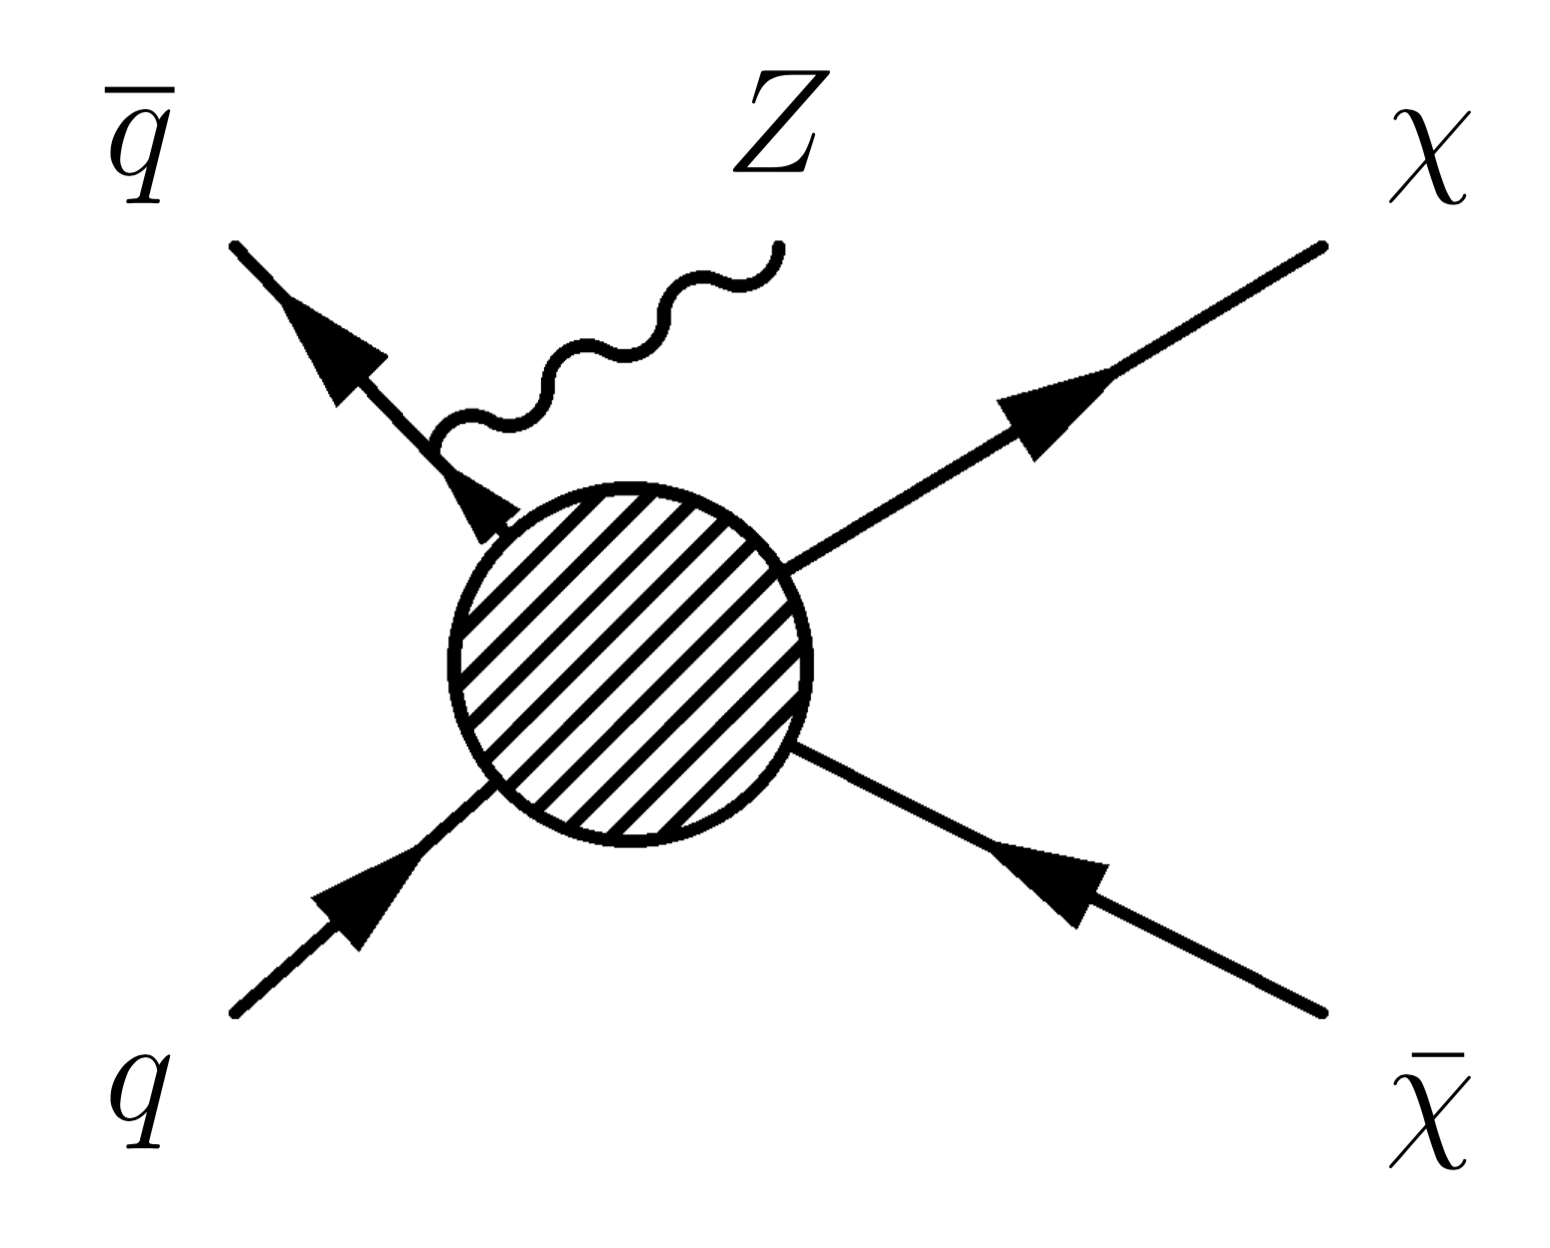
\includegraphics[width=0.3\textwidth]{Figures/eft.png}
% Alison's thesis: https://dspace.library.uvic.ca/handle/1828/8494
\caption{An example EFT with a $Z+\chi\bar{\chi}$ final state with a $Z$ emitted as ISR.}
\label{fig:eft}
\end{figure}

% -------------------------------------------
\subsection{Simplified Models}

Simplified models are the benchmark models used for $E_T^\text{miss}+X$ searches in Run 2. An example $s$-channel diagram for the $E_T^\text{miss}+Z$ signal is shown in Figure \ref{fig:simp}. These models are considered `simplified' because they introduce the minimum number of parameters needed to include a mediator between SM and dark matter particles (compared to more complicated models such as supersymmetry). 

\begin{figure}[htb]
\centering
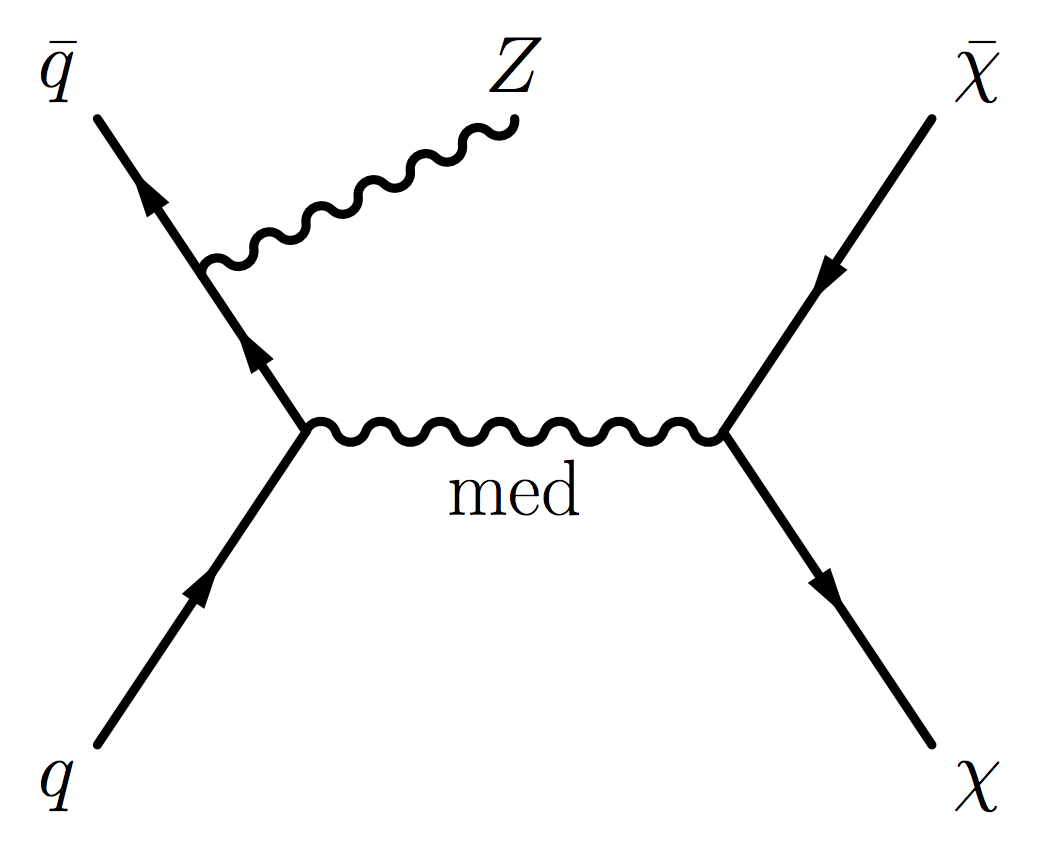
\includegraphics[width=0.375\textwidth]{Figures/simp.png}
% EPS paper: https://arxiv.org/abs/1708.09624
\caption{$s$-channel diagram for WIMP pair production with a $Z$ emitted as ISR.}
\label{fig:simp}
\end{figure}

Simplified models introduce five BSM parameters: the mass of the WIMP, $m_\chi$, the mass of the mediating particle, $m_\text{med}$, the couplings of the mediator to the SM (to dark matter), $g_q$ ($g_\chi$), and the width of the mediator $\Gamma_\text{med}$. The mediator particle can be spin-0 (scalar or pseudo-scalar) or spin-1 (vector or axial-vector). The interaction Lagrangians for models with vector and axial-vector mediator couplings are given in Equations \ref{eqn:Lvector}, and \ref{eqn:Laxial}:

\begin{equation}
\mathcal{L}_\text{vector} = g_q \sum_q \eta_\mu \bar{q} \gamma^\mu q + g_\chi \eta_\mu \bar{\chi} \gamma^\mu \chi
\label{eqn:Lvector}
\end{equation}

\begin{equation}
\mathcal{L}_\text{axial-vector} = g_q \sum_q \eta_\mu \bar{q} \gamma^\mu \gamma^5 q + g_\chi \eta_\mu \bar{\chi} \gamma^\mu \gamma^5\chi
\label{eqn:Laxial}
\end{equation}

\noindent In these equations the mediator is denoted as $\eta$. Following the recommendations of TODO, the couplings are fixed to $g_q = 0.25$ and $g_\chi = 1.0$. In addition, assuming that the mediator has no additional decay modes, $\Gamma_\text{med}$ is set to the so-called minimal width, which is fixed by $g_q$, $g_\chi$, $m_\chi$, and $m_\text{med}$. % https://arxiv.org/pdf/1507.00966.pdf
% Couplings chosen to correspond with rough estimate of lower sensitivity of mono-jet in Run 2, and so that Gamma(med)/m(med) < ~0.05

Similarly, the interaction Lagrangians for models with scalar and pseudo-scalar mediator couplings are given by Equations \ref{eqn:Lscalar} and \ref{eqn:Lpseudo}:

\begin{equation}
\mathcal{L}_\text{scalar} = g_\chi \eta \bar{\chi} \chi + \frac{\eta}{\sqrt{2}} g_q \sum_i \left( y_i^u \bar{u}_i u_i + y_i^d \bar{d}_i d_i + y_i^\ell \bar{\ell}_i \ell_i \right)
\label{eqn:Lscalar}
\end{equation}

\begin{equation}
\mathcal{L}_\text{pseudo-scalar} = i g_\chi \eta \bar{\chi} \gamma_5 \chi + \frac{i \eta}{\sqrt{2}} g_q \sum_i \left( y_i^u \bar{u}_i \gamma_5 u_i + y_i^d \bar{d}_i \gamma_5 d_i + y_i^\ell \bar{\ell}_i \gamma_5 \ell_i \right)
\label{eqn:Lpseudo}
\end{equation}

\noindent For these models, the couplings are set to $g_q = g_\chi = 1.0$, and additional Yukawa couplings $y_i^f$ are introduced that are proportional to the quark masses. 
% Assuming minimal flavour violation, spin-0 resonances will behave similarly to the Higgs boson (hence the Yukawa couplings)

Run 2 analyses have adopted the $s$-channel exchange of an axial-vector mediator as the benchmark scenario. This choice is motivated by the findings in TODO that show that collider searches can be more sensitive than DD experiments at low values of $m_\chi$ for this type of mediator. It should also be noted that, in the time since these initial benchmark models were set, next-to-leading order (NLO) models are now being considered instead of the leading order (LO) tree diagrams discussed here. Finally, in addition to these $s$-channel diagrams there also exist $t$-channel processes that are of great interest to the mono-$Z$ search. These will be discussed more in Chapter \ref{chapter:fullRun2}.

Although they have advantages compared to EFTs, simplified models are not a complete theory, and violate gauge invariance and perturbative unitarity. In Run 2 they have been and will continue to be exceedingly useful in providing a guideline for the ATLAS and CMS collaborations to follow in tandem, but there is now a push towards studying more theoretically complete models.

% -------------------------------------------
\subsection{2 Higgs Doublet + Pseudo-Scalar Model}
% https://arxiv.org/pdf/1701.07427.pdf

A model that is becoming popular in mono-$X$ dark matter searches is known as the two Higgs doublet + pseudo-scalar (2HDM+PS) model. This category of model is self consistent and unitary.

\begin{figure}[htb]
\centering
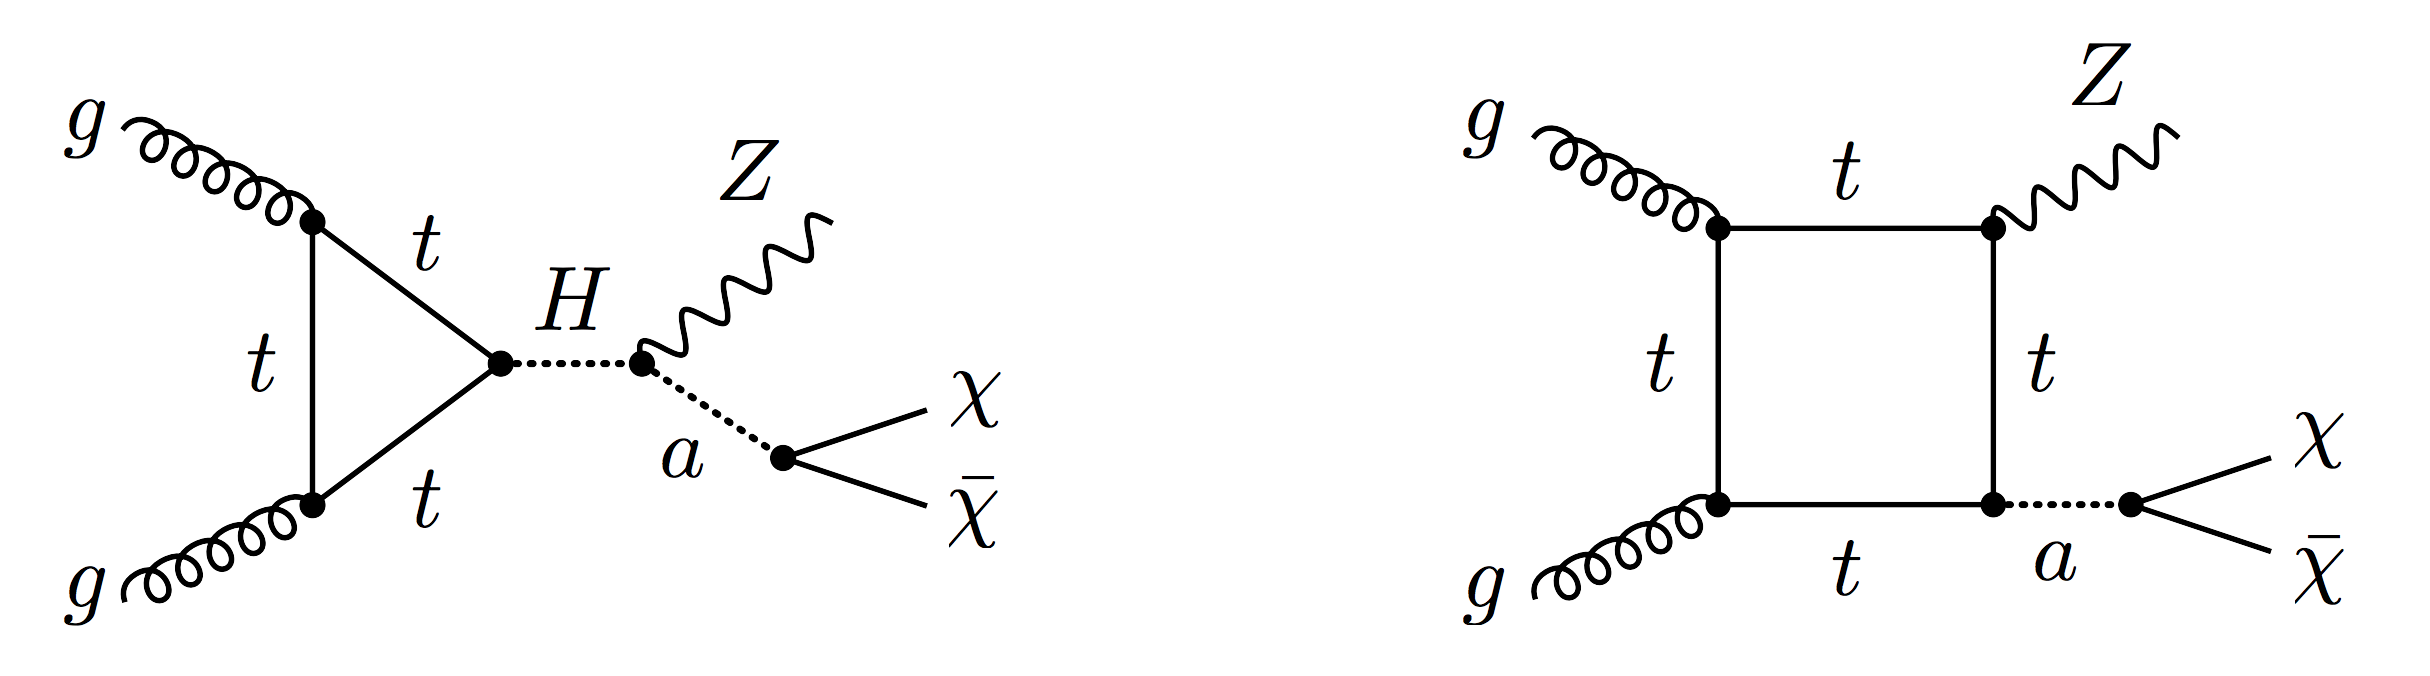
\includegraphics[width=0.75\textwidth]{Figures/2hdma.png}
% EPS paper: https://arxiv.org/abs/1708.09624
\caption{Representative diagrams of the mono-$Z$ signature in the 2HDM+PS model.}
\label{fig:2hdma}
\end{figure}



% --------------------------------------------------------------------------------------
\section{The LHC and the ATLAS Detector}

- introduce the LHC, define luminosity, mention beam energy, beam structure, ...\\
- overview of four main detectors\\
- summary of detector subsystems: inner detector, EM calorimeter, HAD calorimeter, muon spectrometer\\
- trigger, object reconstruction, missing transverse energy\\
- units of cross section\\